\chapter{Materialanhang}

\begin{figure}[ht]
	\centering
	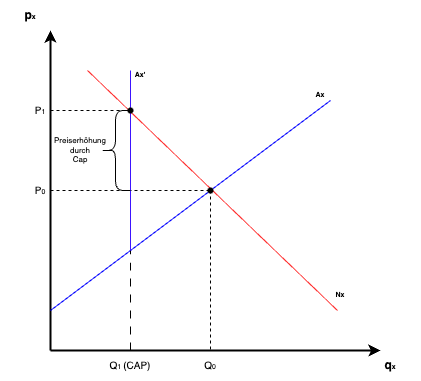
\includegraphics[width=0.8\textwidth]{Bilder/supply_demand_ets.png} 
	\caption{Angebot und Nachfrage von Emissionszertifikaten mit CAP (vgl. \cite{pettinger.2017})}
	\label{fig:supply_demand_ets}
\end{figure}

\begin{figure}[ht]
	\centering
	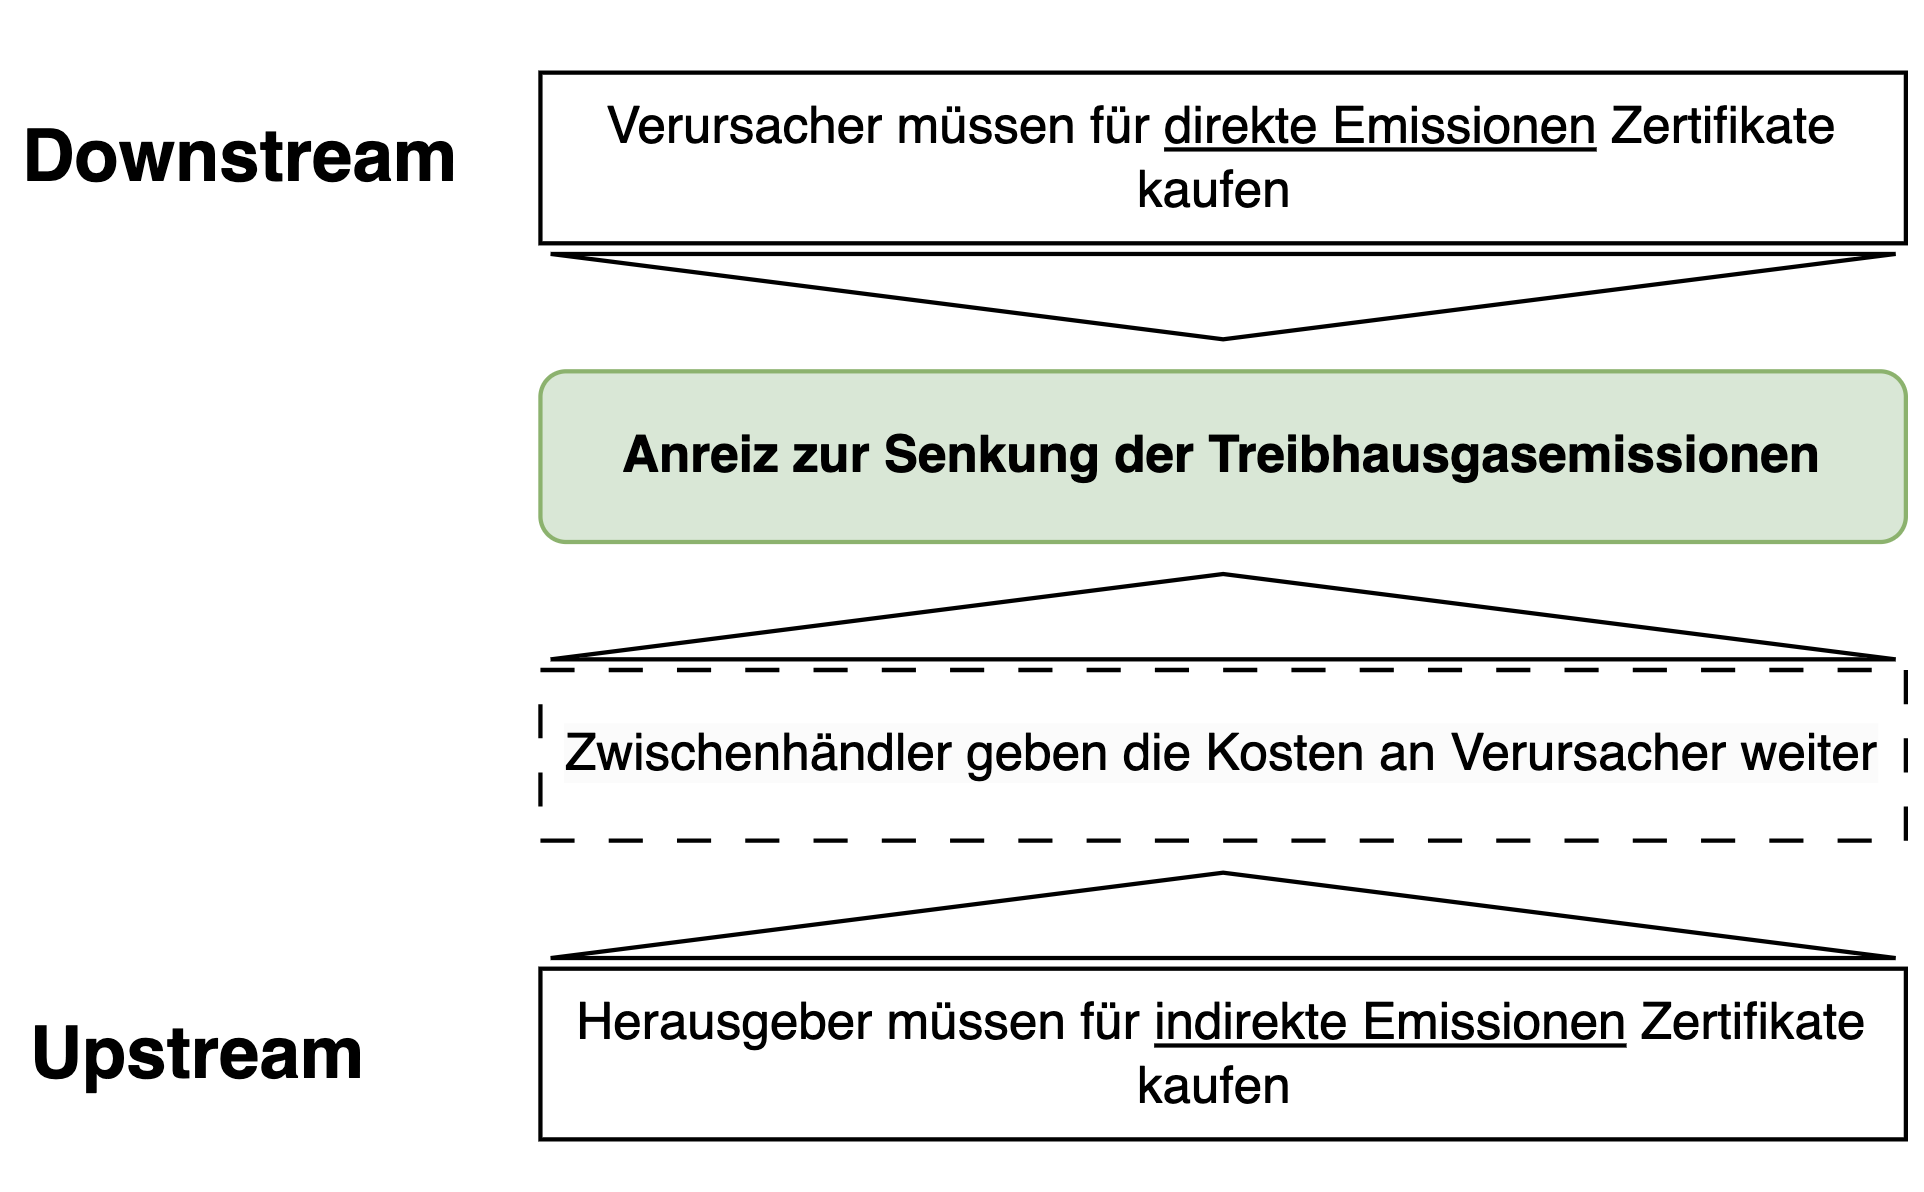
\includegraphics[width=0.8\textwidth]{Bilder/up_and_downstream_ets.png} 
	\caption{Anreize für Verursacher über Upstream- und Downstream-Systeme (vgl. \cite{dehst.2023})}
	\label{fig:up_and_downstream_ets}
\end{figure}

\begin{figure}[ht]
	\centering
	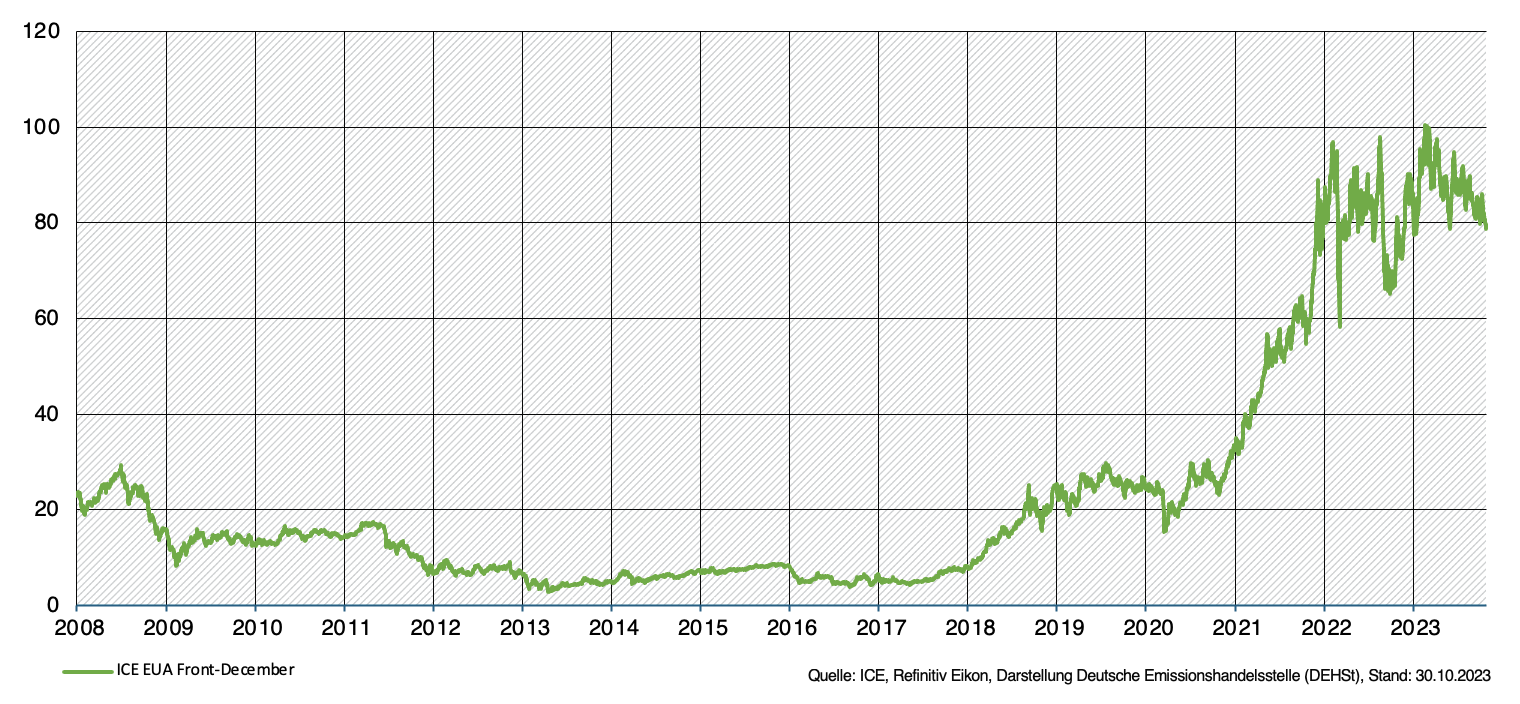
\includegraphics[width=1.0\textwidth]{Bilder/price_co2_eu_ets.png} 
	\caption{Preisentwicklung in € für Emissionsberechtigungen im EU ETS seit 2008 als $CO_2$e-Preis pro Tonne (\cite{dehst.2023})}
	\label{fig:price_co2_eu_ets}
\end{figure}

\begin{figure}[ht]
	\centering
	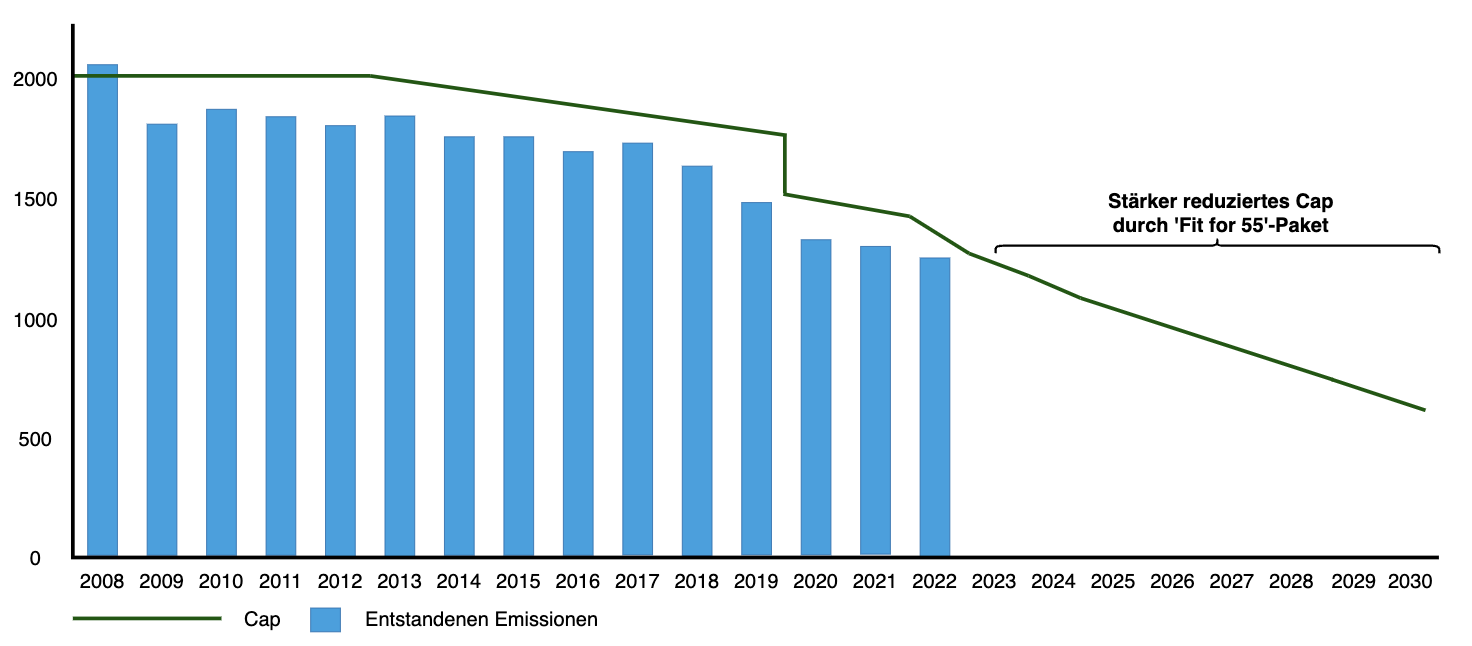
\includegraphics[width=1.0\textwidth]{Bilder/cap_ets.png} 
	\caption{CAP und Emissionen im EU ETS in Mio. Tonnen $CO_2$e (2008-2030) (vgl. \cite{ub3.2023})}
	\label{fig:cap_ets}
\end{figure}

\begin{figure}[ht]
	\centering
	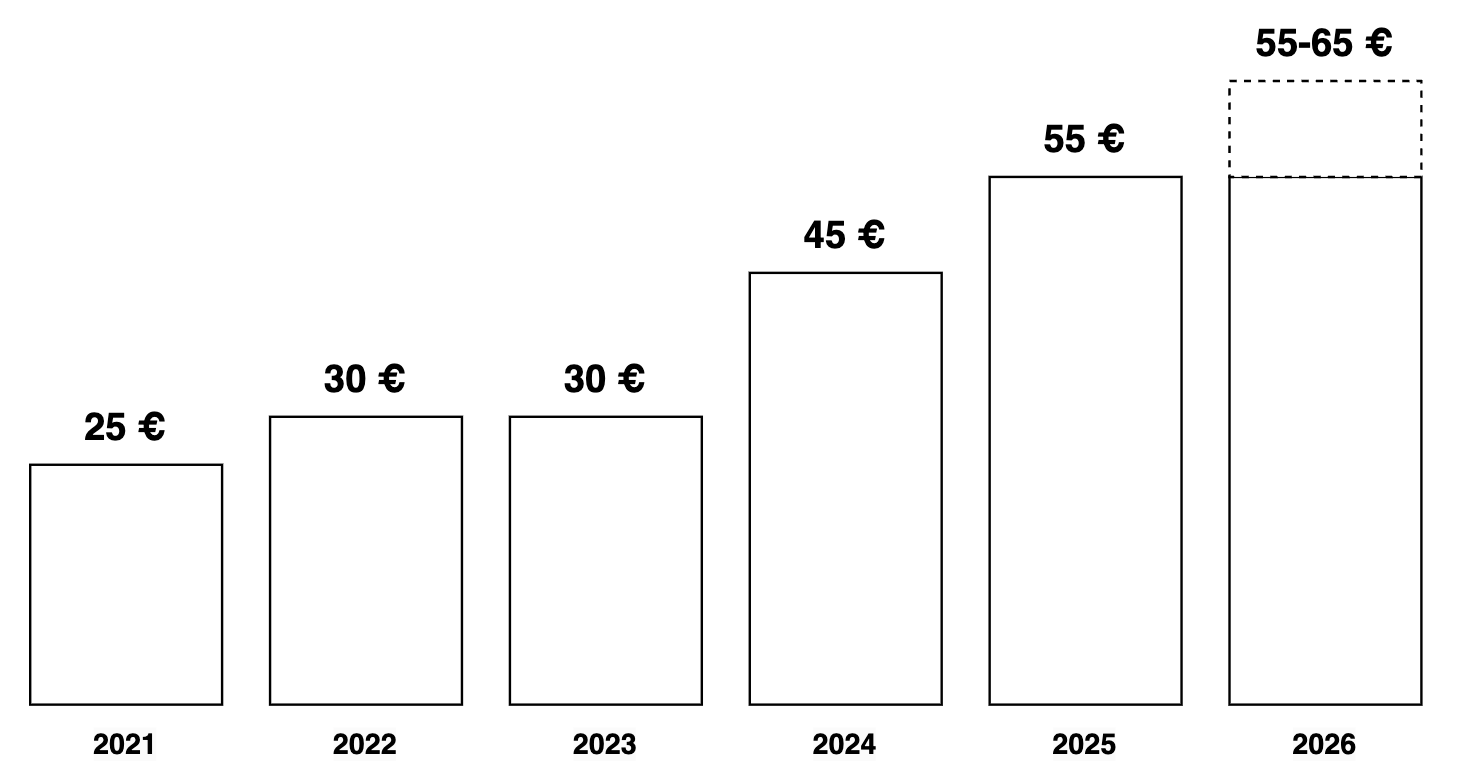
\includegraphics[width=1.0\textwidth]{Bilder/prices_nehs.png} 
	\caption{Preisentwicklung $CO_2$e-Preis pro Tonne für den nEHS (\cite{dehst.2023})}
	\label{fig:prices_nehs}
\end{figure}